\documentclass[11pt, aspectratio=169]{beamer}

\usepackage[utf8]{inputenc}
\usepackage{float}
\usepackage[english]{babel}
\usepackage{tikz-cd}
\usepackage{amsthm}
\usepackage{bbm}
\usepackage{amsmath}
\usepackage{amsfonts}
\usepackage{amssymb}
\usepackage{mathtools}
\usepackage{graphicx}
\usepackage{rotating}
\usepackage{setspace}
\usepackage{color}
\usepackage{fancyhdr}
\usepackage{ragged2e}
\usepackage{appendix}
\usepackage{tabularx}
\usepackage{multirow}
\usepackage{booktabs}
\usepackage{xfrac}
\usepackage{pgfplots}
\usepackage{url}
\usepackage{emptypage}
\usepackage{wrapfig}
\usepackage{dsfont}
\usepackage{makecell}
\usepackage{bm}
\usepackage{csquotes}




\pgfplotsset{compat=1.18}

% \usepackage{tikz-cd}
% \usepackage{indentfirst}
% \usecolortheme{default}
% \usepackage{color}
% %\usepackage{newtxmath}
% \setbeamercovered{dynamic}
% \usepackage{multirow}
% \usepackage{amsfonts}
% \usepackage{amssymb}
% \usepackage{graphicx}
% \usepackage{amsmath}
% \usepackage{bm}
% \usepackage{faktor}
% \usepackage{amsthm}
% \usepackage{calrsfs}
% %\usepackage{etoolbox}
% \usepackage{commath}
% %\usepackage{mathtools}
% \usepackage{imakeidx}
% \makeindex
% \usepackage{dsfont}
% \usepackage{breqn}
% \usepackage{xfrac}
% \usepackage{braket}
% %\usepackage{wrapfig}


%Operators
\DeclareMathOperator{\CVar}{CVar}
\DeclareMathOperator{\Span}{Span}

%shortcuts
\newcommand{\nc}{\newcommand} 
\nc{\cH}{{\mathcal H}}
\nc{\cR}{{\mathcal R}}
\nc{\cA}{{\mathcal A}}
\nc{\cG}{{\mathcal G}}
\nc{\cC}{{\mathcal C}}
\nc{\cD}{{\mathcal D}}
\nc{\cO}{{\mathcal O}}
\nc{\cI}{{\mathcal I}}
\nc{\cB}{{\mathcal B}}
\nc{\cY}{{\mathcal Y}}
\nc{\cK}{{\mathcal K}} 
\nc{\cX}{{\mathcal X}}
\nc{\cS}{{\mathcal S}}
\nc{\cE}{{\mathcal E}}
\nc{\cF}{{\mathcal F}}
\nc{\cZ}{{\mathcal Z}}
\nc{\cQ}{{\mathcal Q}}
\nc{\cN}{{\mathcal N}}
\nc{\cP}{{\mathcal P}}
\nc{\cL}{{\mathcal L}}
\nc{\cM}{{\mathcal M}}
\nc{\cT}{{\mathcal T}}
\nc{\cW}{{\mathcal W}}
\nc{\cU}{{\mathcal U}}
\nc{\cJ}{{\mathcal J}}
\nc{\cV}{{\mathcal V}}
\nc{\bH}{{\mathbb H}}
\nc{\bA}{{\mathbb A}}
\nc{\bG}{{\mathbb G}}
\nc{\bC}{{\mathbb C}}
\nc{\bO}{{\mathbb O}}
\nc{\bI}{{\mathbb I}}
\nc{\bB}{{\mathbb B}}
\nc{\bY}{{\mathbb Y}}
\nc{\bK}{{\mathbb K}} 
\nc{\bX}{{\mathbb X}}
\nc{\bS}{{\mathbb S}}
\nc{\bE}{{\mathbb E}}
\nc{\bF}{{\mathbb F}}
\nc{\bZ}{{\mathbb Z}}
\nc{\bQ}{{\mathbb Q}}
\nc{\bN}{{\mathbb N}}
\nc{\bP}{{\mathbb P}}
\nc{\bL}{{\mathbb L}}
\nc{\bM}{{\mathbb M}}
\nc{\bT}{{\mathbb T}}
\nc{\bW}{{\mathbb W}}
\nc{\bU}{{\mathbb U}}
\nc{\bD}{{\mathbb D}}
\nc{\bJ}{{\mathbb J}}
\nc{\bV}{{\mathbb V}}
\nc{\bR}{{\mathbb R}}

\nc{\boB}{{\mathbf{B}}}
\nc{\boL}{{\mathbf{L}}}
\nc{\boG}{{\mathbf{G}}}


\nc{\tV}{{\Tilde{{V}}}}
\nc{\tI}{{\Tilde{{I}}}}
\nc{\tY}{{\Tilde{{Y}}}}
\nc{\tS}{{\Tilde{{S}}}}

\nc{\fr}{{\rightarrow}}
\nc{\co}{{\nabla}}

\newcommand{\la}{\; \longrightarrow \;}
\nc{\cu}{{\barline{\nabla}}}



%%MATH OPERATORS

\DeclareMathOperator{\diag}{diag}
\DeclareMathOperator{\cost}{c}
%%MODEL COMMANDS
\nc{\Vv}{{\mathbf{u}}}
\nc{\Yv}{{\mathbf{Y}}}
\nc{\Sv}{{\mathbf{S}}}
\nc{\conj}[1]{\overline{#1}}

%%Graph
\nc{\netNodes}{\cB}
\nc{\netEdges}{\cL}

%%
\nc{\PFspace}{\mathcal{X}_{\text{PF}}}
% % Custom colors
% \usepackage{color}
% \definecolor{deepblue}{rgb}{0,0,0.5}
% \definecolor{deepred}{rgb}{0.6,0,0}
% \definecolor{deepgreen}{rgb}{0,0.5,0}

% \usepackage{listings}

% \definecolor{codegreen}{rgb}{0,0.6,0}
% \definecolor{codegray}{rgb}{0.5,0.5,0.5}
% \definecolor{codepurple}{rgb}{0.58,0,0.82}
% \definecolor{backcolour}{rgb}{0.95,0.95,0.92}

% % Python style for highlighting
% \newcommand\pythonstyle{\lstset{
% language=Python,
% basicstyle=\ttm,
% morekeywords={self},              % Add keywords here
% keywordstyle=\ttb\color{deepblue},
% emph={MyClass,__init__},          % Custom highlighting
% emphstyle=\ttb\color{deepred},    % Custom highlighting style
% stringstyle=\color{deepgreen},
% frame=tb,                         % Any extra options here
% showstringspaces=false
% }}


% % Python environment
% \lstnewenvironment{python}[1][]
% {
% \pythonstyle
% \lstset{#1}
% }
% {}

% % Python for external files
% \newcommand\pythonexternal[2][]{{
% \pythonstyle
% \lstinputlisting[#1]{#2}}}

% % Python for inline
% \newcommand\pythoninline[1]{{\pythonstyle\lstinline!#1!}}



\usepackage[
backend=biber,
style=alphabetic,
sorting=nty
, maxbibnames=99]{biblatex}

\addbibresource{sample.bib}




\usepackage{ragged2e} % giustifica
\justifying
\setbeamertemplate{caption}{\insertcaption}
\setbeamercovered{invisible}
%\setbeamertemplate{footline}[frame number]
\usepackage{tikz}
\usetikzlibrary{arrows,%
                shapes,positioning}
                
                \definecolor{blendedblue}{rgb}{0.2,0.2,0.7}
        
\usetikzlibrary{%
                petri,%
                topaths}%
%\usepackage{tikz-berge}


\usepackage{ifpdf} 
\ifpdf% 
        \usepackage{pdftricks} 

        \begin{psinputs} 
            \usepackage{pstricks} 
            \usepackage{pstricks-add} 
            \usepackage{pst-plot} 
            \usepackage{pst-text,pst-node,pst-tree} 
        \end{psinputs} 
\else 
        \usepackage{pstricks} 
        \usepackage{pstricks-add} 
        \usepackage{pst-plot} 
        \usepackage{pst-text,pst-node,pst-tree} 

\fi 

\usepackage{pstricks}

\makeatletter
\setbeamertemplate{footline}
{
  \leavevmode%
  \hbox{%
  \begin{beamercolorbox}[wd=.333333\paperwidth,ht=2.25ex,dp=1ex,left]{author in head/foot}%
    \usebeamerfont{author in head/foot}\hspace*{2ex}\insertauthor
  \end{beamercolorbox}%
  \begin{beamercolorbox}[wd=.333333\paperwidth,ht=2.25ex,dp=1ex,center]{title in head/foot}%
    \usebeamerfont{title in head/foot}\insertsubsection
  \end{beamercolorbox}%
  \begin{beamercolorbox}[wd=.333333\paperwidth,ht=2.25ex,dp=1ex,right]{date in head/foot}%
    \usebeamerfont{date in head/foot}\insertshortdate{}\hspace*{2em}
    \insertframenumber{} / \inserttotalframenumber\hspace*{2ex} 
  \end{beamercolorbox}}%
  \vskip0pt%
}
\makeatother
\setbeamertemplate{navigation symbols}{}

\usepackage{color}
\definecolor{deepblue}{rgb}{0,0,0.5}
\definecolor{deepred}{rgb}{0.6,0,0}
\definecolor{deepgreen}{rgb}{0,0.5,0}

\usepackage{listings}

\definecolor{codegreen}{rgb}{0,0.6,0}
\definecolor{codegray}{rgb}{0.5,0.5,0.5}
\definecolor{codepurple}{rgb}{0.58,0,0.82}
\definecolor{backcolour}{rgb}{0.95,0.95,0.92}

\lstdefinestyle{mystyle}{
    backgroundcolor=\color{backcolour},   
    commentstyle=\color{codegreen},
    keywordstyle=\color{magenta},
    numberstyle=\tiny\color{codegray},
    stringstyle=\color{codepurple},
    basicstyle=\ttfamily\footnotesize,
    breakatwhitespace=false,         
    breaklines=true,                 
    captionpos=b,                    
    keepspaces=true,                 
    numbers=left,                    
    numbersep=5pt,                  
    showspaces=false,                
    showstringspaces=false,
    showtabs=false,                  
    tabsize=2
}

\lstset{style=mystyle}


\newtheorem{prop}[theorem]{Proposition}
\newtheorem{defi}[theorem]{Definition}
\newtheorem{oss}[theorem]{Observation}
\newtheorem{theo}[theorem]{Theorem}
\newtheorem{cor}[theorem]{Corollary}
\newtheorem{assumption}[theorem]{Assumption}
\renewcommand*{\bibfont}{\footnotesize}

\title{Optimization problems in Power Systems}
\author{Gabor Riccardi}
\date{\today}
%\institute{Università degli Studi di Pavia}
\institute{Università di Pavia}
% - Dipartimento di Matematica "Felice Casorati"


\begin{document}
%\section{AC-OPF Models}
\begin{frame}[plain]
\centering

\includegraphics[scale=0.5]{unipv.png}
\maketitle
\end{frame}

\begin{frame}{Optimal Power Flow problems}
    \begin{figure}
        \centering
        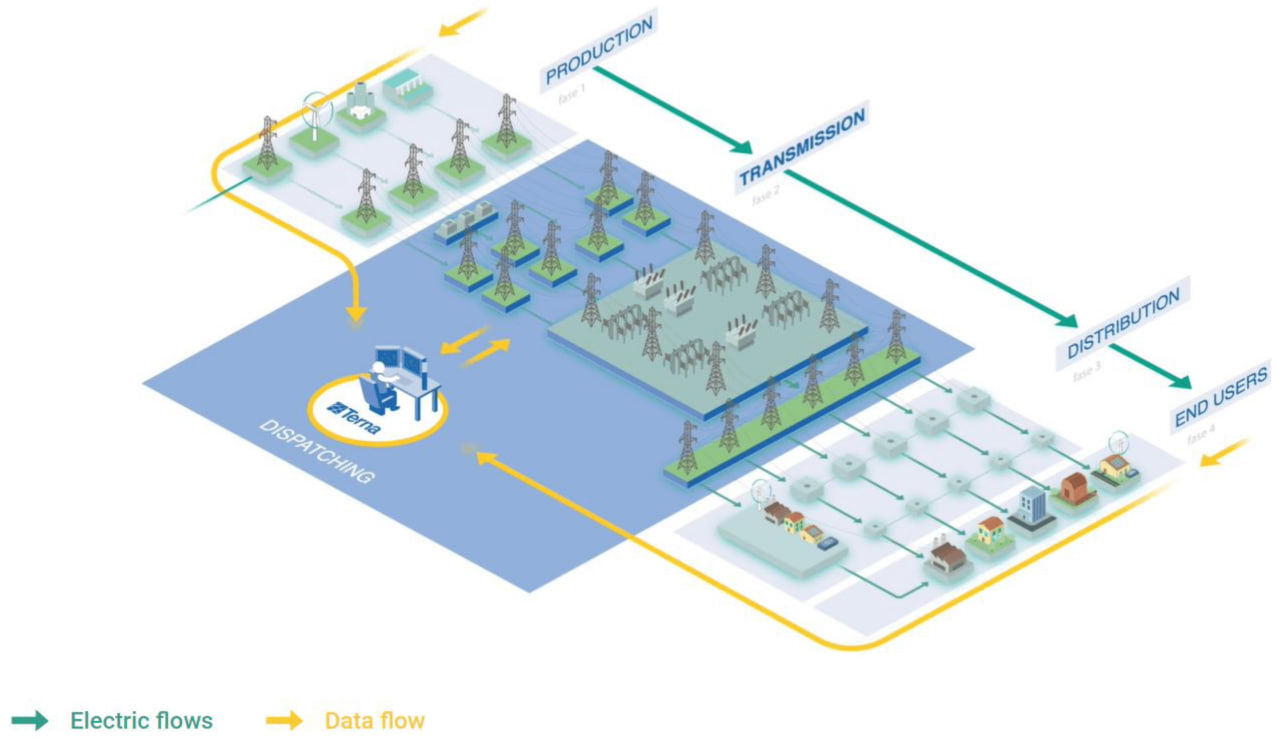
\includegraphics[width=0.8\textwidth]{photo_2023-09-26_14-27-16.jpg}
        \label{fig:enter-label}
    \end{figure}
\end{frame}


\begin{frame}
	\tableofcontents
\end{frame}




%  \begin{frame}


% Optimal Power Flow (OPF) is the set of optimization problems in electric power systems engineering which seek to optimize the operation of an electrical power system subject to the physical constraints imposed by electrical laws and engineering limits.\\[2em] 

% \begin{itemize}
%     \item Deterministic optimal power flow models: solved in real-time scenarios.\\[2em] 
%     \item Stochastic optimal power flow models: take into account errors in the prediction of loads and of power production of renewable energy sources. Solved for day-ahead marked.
% \end{itemize}
% \end{frame}
\section{AC-OPF formulations}
\begin{frame}{Compact formulation}
\begin{align}
\inf_{\Vv,\Sv \in \bC^{\netNodes}}& \cost(\Vv,\Sv) \\
\text{s.t.} & \nonumber \\
&\diag(\conj{\Vv})\Yv\Vv = \Sv \\
& \underline{\Vv} \leq \overline{\Vv} \\
& \underline{\Sv} \leq \overline{\Sv}
\end{align}
\end{frame}


\begin{frame}{Polar OPF formulation}
% \textcolor{red}{\tiny dire che la f.o. è legata al consumo, parlare in generale dei vincoli dicendo sostanzialmente quello che hai scritto e dire perché il problema è difficile, non convesso NP hard ecc}
%There are various equivalent formulations of the deterministic OPF problem. The Polar formulation is as follows:
\scriptsize
\begin{align}
\label{polar}
\inf_{\substack{P^G_g, Q^G_g, \delta_k \\ |V|_k, S_{km}}}
& \sum_{g \in \mathcal{G}} F_g(P_g^G) \\[1em]
\text{Subject to:} & \nonumber \\
& \text{Voltage to Power Flow constraints:} \quad \forall km \in \boL  \nonumber \\
& S_{km} = (G_{kk}-iB_{kk})|V_k|^2 + (G_{km}-jB_{km})|V_k||V_m|(\cos(\delta_k-\delta_m) + j\sin(\delta_k-\delta_m))  \\[1em]
& \text{Power balance constraints:} \nonumber \\
& \sum_{km \in \delta(k)}S_{km} = (\sum_{g \in \mathcal{G}(k)}P_g^g-P_k^d) + i(\sum_{g \in \mathcal{G}(k)}Q_g^G-Q_k^L) \\[1em]
& \text{Power flow, Voltage, and Power generation limits:} \nonumber \\
& |S_{km}|^2 \leq U_{km}, \quad V_k^{\text{min}} \leq |V_k| \leq V_k^{\text{max}}, \quad P_g^{\text{min}} \leq P_g^G \leq P_g^{\text{max}} \\
& \theta_{km}^{\text{min}} \leq \delta_k - \delta_m \leq \theta_{km}^{\text{max}}
\end{align}

%We note that the cost function is not linear and constraint (2) is not convex, and also the power flow bound is generally quite loose.
\end{frame}

\section{Optimization methods}
\begin{frame}{Methods for Solving AC-OPF}
    \textbf{1. Classical Methods}
    \begin{itemize}
        \item \textbf{Newton-Raphson}: Iterative, relies on solving nonlinear equations.
        \item \textbf{Interior Point Methods (IPMs)}:
        \begin{itemize}
            \item Solve Karush-Kuhn-Tucker (KKT) conditions.
            \item Efficient for large-scale systems.
        \end{itemize}
    \end{itemize}
    
    \textbf{2. Relaxation Techniques}
    \begin{itemize}
        \item \textbf{Semidefinite Programming (SDP)}:
        \begin{itemize}
            \item Convex relaxation.
            \item Provides bounds on global optimum.
        \end{itemize}
        \item \textbf{Second-Order Cone Programming (SOCP)}:
        \begin{itemize}
            \item Weaker relaxation than SDP.
            \item Faster, scalable for large systems.
        \end{itemize}
        \item \textbf{Quadratic Programming (QP)}:
        \begin{itemize}
            \item Linearizes power flow equations.
        \end{itemize}
    \end{itemize}
\end{frame}

\begin{frame}{Global Optimization Techniques}
    \textbf{3. Global Optimization Methods}
    \begin{itemize}
        \item \textbf{Branch-and-Bound}:
        \begin{itemize}
            \item Systematically explores subproblems.
            \item Guarantees global solution.
        \end{itemize}
        \item \textbf{Heuristics}:
        \begin{itemize}
            \item Genetic Algorithms, Simulated Annealing.
            \item Useful for obtaining good feasible solutions.
        \end{itemize}
    \end{itemize}
\end{frame}

\begin{frame}{Conclusion}
    \textbf{Choosing a Method}:
    \begin{itemize}
        \item \textbf{Classical methods}: Efficient but may converge to local optima.
        \item \textbf{Relaxations}: Provide bounds but not always feasible solutions.
        \item \textbf{Global methods}: "Ensure" global optimality but computationally intensive.
    \end{itemize}
    
    \textbf{Trade-off between accuracy and computational effort.}
\end{frame}

\end{document}
 

\begin{frame}{Jabr relaxation}
% \textcolor{red}{\tiny ha avuto particolare successo un rilassamento polinomiale ecc}
Let $\theta_{km} \coloneqq \delta_k - \delta_m$. We can obtain a polynomial relaxation with the following substitutions:

\begin{align}
c_{kk} &\coloneqq |V_k|^2 \\
c_{km} &\coloneqq |V_k||V_m|\cos{\theta_{km}} \\
s_{km} &\coloneqq |V_k||V_m|\sin{\theta_{km}}
\end{align}

% And the following constraints:

% \begin{align}
%     \onslide<2->{|V_k||V_m|\cos{\theta_{km}}^2 + |V_k||V_m|\sin{\theta_{km}}^ 2 = |V_k|^2|V_m|^2 \implies & c_{km}^2 + s_{mk}^2 = c_{ii}c_{jj} \\}
%     \onslide<3->{|V_k|^2 \geq 0 \implies & c_{kk} \geq 0 \\}
%     \onslide<4->{\sin \; (\cos) \text{ is asymmetric (symmetric) } \implies & s_{km}= -s_{mk}, \;  c_{km} = c_{mk} \\}
%     \notag
% \end{align}

\end{frame}


\begin{frame}{Jabr relaxation}
% \textcolor{red}{\tiny che trasforma il modello così, come vedete dal vincolo tal dei tali adesso il modello non è più così ma è cosà}
\scriptsize
\begin{align}
\label{2-jabr}
\inf_{\substack{P^G_g, Q^G_g \\ c_{km},s_{km}}} & \sum_{g \in \mathcal{G}} F_g(P_g^G) \\[1em]
\text{Subject to:} & \nonumber \\
\label{c constraints}
& c_{km}^2 + s_{mk}^2 = c_{ii}c_{jj}, \quad c_{ii} \geq 0, \quad c_{km}=c_{mk}, \quad s_{km}= - s_{mk} \\
& P_{km} = G_{kk}c_{kk}+G_{km}c_{km}+B_{km}s_{km} \\
& Q_{km} = -B_{kk}c_{kk}-B_{km}c_{km}+G_{km}s_{km} \\[1em]
& \text{Power balance constraints:} \nonumber \\
& S_{km} = P_{km} + iQ_{km} \\
& \sum_{km \in \delta(k)}S_{km} = (\sum_{g \in \mathcal{G}(k)}P_g^g-P_k^d) + i(\sum_{g \in \mathcal{G}(k)}Q_g^G-Q_k^L) \\[1em]
& \text{Power flow, Voltage, and Power generation limits:} \nonumber \\
& P_{km}^2 + S_{km}^2 \leq U_{km}, \, V_k^{\text{min}} \leq |V_k| \leq V_k^{\text{max}}, \, P_g^{\text{min}} \leq P_g^G \leq P_g^{\text{max}}
\end{align}

    
\end{frame}



\section{What is known about the AC-OPF feasible space?}

\begin{frame}{What is known (not much)}
\begin{itemize}
\item Not much!
\item Invertibility conditions of admittance matrix (Needed for Newton methods)
\item The feasible space \(\PFspace\) (without magnitude constraints) is a manifold (differentiable? \(C^{inf}\)?)
\item \(\PFspace\) can be disconnected
\item Finding feasible solutions is NP-hard(?)
\item Tangent space of \(PFspace\) is known.
\end{itemize}
\end{frame}




\end{document}








